In this chapter I'm gonna put all stuff about generative field. I'd lie to speak about GANs network and other advanced stuff but before I need to put together some backgrounds concepts like Boltzman machine Energy-based model and so on. 

\section{Energy based model}
%This is an extract of the presentation \textit{https://deepgenerativemodels.github.io/assets/slides/cs236\_lecture11.pdf}
Let's say that a probability function $p(x)$ needs to respects this rules:
\begin{itemize}
 \item $\forall x, p(x) >= 0$ 
 \item $\sum_x p(x) = 1$
 \end{itemize} 
 You can have a more deep definition in the probability chapter.
 In order to define this $p(x)$ function we need to guarantee the respect of those constrains. Let's imagine $p(x) = x^2$
 In this case the first rule is respected but not the second, so this function can be used. So, to use a positive function we need to normalize it. Let's define $p'(x)$ as the normalized version of $p(x)$ in order to respect both the rule:
 \begin{equation}
 p'(x) = \frac{p(x)}{\int p(x)dx}
 \end{equation}\label{normalizationfunctionforprobability}
 We have normalized $p(x)$ by the area above the the function.
 
 Now we can define  the probability function $p(x)$ the function:
 \begin{equation}
 p(x) = \frac{exp(f(x)}{\int exp(f(x))dx}
 \end{equation}
 We can define:
 \begin{equation}
 Z = \int exp(f(x))dx
 \end{equation}
 As you can see it was used $exp()$ function in order to guarantee the first rule. Furthermore this function allow to better capture variations, many distribution can be written in exponential form.
 
 In this system we can call $f(x)$ the \textbf{The energy function} and we see the method to turn it in to a probability function
 
\subsection{How it work?}
 The \textbf{Energy based model} has to associate to each configuration of the input variables a scalar that indicates how much energy has this configuration. A good configuration has low energy, so a low value while a bad one has a greater energy.
 
 For example let's say we have in imagine $M$ and a set of object $(s_0, s_1,.. s_5)$. The imagine contains one object from the set and we want create a model capable to identify it. Let's say that we want a model capable to give to the right $s_i$ lesser energy than the other.
 
  %https://rubikscode.net/2018/10/01/introduction-to-restricted-boltzmann-machines/
 \section{Boltzman Machine}
 \begin{figure}
  \centering
    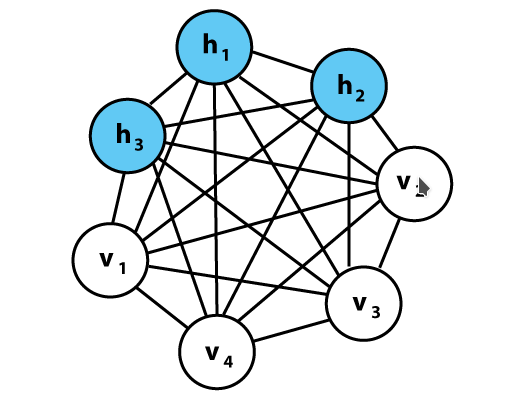
\includegraphics[scale=0.65]{img/boltzmanMachine.png}
    \caption{boltzman machine model}
    \label{img:bolzman_machine}
 \end{figure}
 Boltzman machine is a symmetrically  connected neurons model. Each of these neurons has a binary state so they can be on or off.
 A Boltzman machine is composed by nodes, called, neurons, connected to the others with a weighted connection. Nodes can be visible of hidden. This means the user will be able to set input in the visible neurons not in the hidden ones.
 
 Each neurons compute its state according to a probability function that means the probability of the neuron to change state:
 
 \begin{equation}
 prob(s_i = 1) = \frac{1}{1 + e^{-z_i}}
 \end{equation}
 
 As we can see this formula uses a parameter $z_i$ that is computed by summing all weighted states of input nodes plus a bias:
 
 \begin{equation}
 z_i = b_i + \sum_{j} s_j w_{ij}
 \end{equation}
 
 Now, once all nodes are update, we can compute the \textbf{Energy of the system} using a \textbf{Boltzman Distribution} that is a energy probability function for discrete value.
 
 Let's define $\vec{v}$ the vector containing all states and $\mathbb{U}$ all the possible state vectors. Now we can compute the probability of the system using:
 \begin{equation}
 P(\vec{v}) = \frac{exp(-E(\vec{v}))}{\sum_{\vec{u}\in\mathbb{U}} exp(-E(\vec{u}))}
 \end{equation}

$E()$ is the boltzman energy function:
\begin{equation}
E(\vec{v}) = - \sum_i s_i^v b_i - \sum_{i < j} s_i^v s_j^v w_{ij}
\end{equation}

The goal of this machine is to set weighs in order to minimize the energy of the system for the right configuration of states, and maximize it for the wrong configuration.
\textbf{Problems:} Nodes are all connected to each other and that makes the model learning really long. That why \textbf{Restricted Boltzman Machines (RBM)} came into the picture

\subsection{Restricted Boltzman Machine}
\begin{figure}
  \centering
    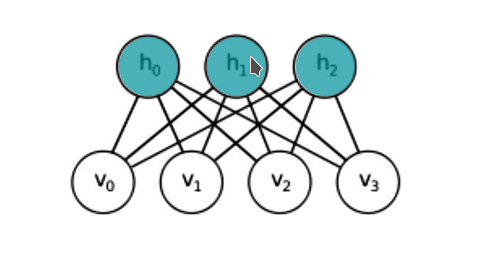
\includegraphics[scale=0.65]{img/RestrictedBoltzmanMachine.png}
    \caption{restricted boltzman machine model}
    \label{img:restricted_bolzman_machine}
 \end{figure}
 The main difference between Boltzman Machine and Restricted Boltzman Machine is that visible nodes are link just to hiddens one and viceversa. Less connections less learning time. The State vector $\vec{v'}$ is composed by the visible state vector $\vec{v}$ and the hidden vector $\vec{h}$. The energy is computed:
 \begin{equation}
 E(v,h) = - \sum_{i} a_iv_i - \sum_j b_j h_j - \sum v_i h_i w_ij
 \end{equation}
Where $a_i$ and $b_i$ are the bias. The probability of the system can be expressed as:
\begin{equation}
p(v,h) = \frac{exp(-E(v,h))}{\sum_{v,h} exp(-E(v,h))}
\end{equation}
Now it si possible to calculate the probability of a single hidden neuron to be activated:
\begin{equation}
p(h_j = 1 | v) = \frac{1}{1 + exp(-(b_j+W-jv_j))} = \sigma (a_i + \sum_j h_j w_ij)
\end{equation}

As we can see from the above equation it can be expressed as a logistic function